\documentclass[11pt]{article}

\usepackage[utf8]{inputenc}
\usepackage[T1]{fontenc}
\usepackage{amsmath,amssymb,amsthm}
\usepackage{hyperref}
\usepackage{graphicx}
\usepackage{geometry}
\geometry{margin=2.5cm}
\usepackage{tikz}
\usepackage{pgfmath}

\newtheorem{theorem}{Theorem}

\title{Trigonometry without $\pi$: a constructive approach}
\author{Daniel de Rauglaudre (alias roglo)}
\date{\today}

\begin{document}

\maketitle

\begin{abstract}
We present a construction of trigonometry where angles are not real
numbers, but pairs $(x,y)$ such that $x^2 + y^2 = 1$. Several classic
trigonometric formulas naturally emerge during this construction,
which leads to defining the division of an angle by an integer using a
convergent sequence. This construction does not require the prior
definition of the constant $\pi$, which is never used. All results are
formally proven using the Coq proof assistant.
\end{abstract}

\section{Introduction}

... to be done ...

\section{Basic Construction}

In classical trigonometry, angles are real numbers. The set \( A \) of
angles is therefore defined by

\[
A ::= \mathbb{R}
\]

\noindent Here, we will forget this definition and instead define

\[
A ::= \{ \; (x, y) \; | \; x^2 + y^2 = 1 \; \}
\]

\noindent In other words, an angle is defined by a point on the unit
circle. This represents the angle between the positive \( x \)-axis
and the line segment joining the origin \( O \) and the given point.

\

\noindent Here, the angle $(x, y)$

\

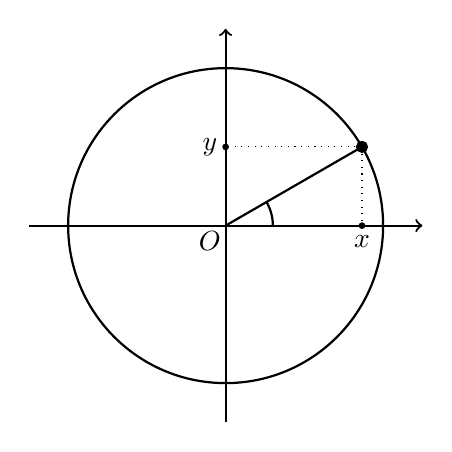
\begin{tikzpicture}
    \draw[thick] (0,0) circle(2);

    \draw[->, thick] (-2.5, 0) -- (2.5, 0);
    \draw[->, thick] (0, -2.5) -- (0, 2.5);

    \node at (-0.2,-0.2) {$O$};

    \pgfmathsetmacro{\px}{cos(30)}
    \pgfmathsetmacro{\py}{sin(30)}
    \coordinate (P) at (\px*2, \py*2);
    \draw[fill] (P) circle (2pt);

    \draw[thick] (0,0) -- (P);

    \draw[thick] (0.6,0) arc[start angle=0, end angle=30, radius=0.6];

    \draw[dotted] (P) -- (\px*2, 0);
    \draw[fill] (\px*2, 0) circle (1pt);
    \node at (\px*2, -0.2) {$x$};

    \draw[dotted] (P) -- (0, \py*2);
    \draw[fill] (0, \py*2) circle (1pt);
    \node at (-0.2, \py*2) {$y$};

\end{tikzpicture}

\

\

\noindent An angle $\theta$ is therefore not a real, but a triplet

$\theta = (x, y, x^2\!+\!y^2\!=\!1)$

\

\noindent In that case, we define

$cos(\theta) = x$

$sin(\theta) = y$

\

\noindent These are our {\em definitions} of cos and sin. The third
component of $\theta$ is a proof that $x^2+y^2=1$. Note that, in
traditional mathematics, proofs are not mathematical objects. Here, we
work in Type Theory where proofs are themselves mathematical
objects. And now, a first theorem

\begin{theorem}
$\cos^2(\theta) + \sin^2(\theta) = 1$.
\end{theorem}

\begin{proof}
By definition of angles, this is this third component.
\end{proof}

\

\noindent Note that in classical trigonometry, this theorem must be
proven using the definitions of $cos$ and $sin$, which are
series. Here, we don't need that, the result is straightforward.

\

\noindent The same way, here, $cos$ and $sin$ are directly accessed
from the angle. In classical trigonometry, being series, they even
cannot be computed: they are just limits of the series seen as
sequences. For example, there is no algorithm computing $sin(0)$: they
can just can claim that the $sin$ of $0$ is indeed $0$, i.e. the limit
of the series $sin$ in $0$ is indeed $0$. In classical trigonometry,
$sin$ and $cos$ are functions in mathematical sense, not in
programming sense.

\

...

\section{Conclusion}

... to be done ...

\paragraph{Code source :}
\url{https://github.com/roglo/coq_sensitivity/tree/master/trigo_without_pi}

\end{document}
